\documentclass[a4paper,12pt,parskip]{scrartcl}

\linespread{1.25}

\usepackage{lmodern}

\usepackage{csquotes}
\usepackage[english]{babel}

\usepackage{xcolor}
\usepackage{float}
\usepackage{listings}

\usepackage[export]{adjustbox}

\lstset{
  basicstyle         = \ttfamily,
  breaklines         = true,
  showstringspaces   = false,
  commentstyle       = \color{red},
  keywordstyle       = \color{blue},
  rangeprefix        = \#\#\#\ ,
  rangebeginsuffix   = \ begin,
  rangeendsuffix     = \ end,
  includerangemarker = false,
}

\usepackage[
  style   = numeric,
  sorting = none,
]{biblatex}
\bibliography{thesis}

\usepackage[toc,page]{appendix}
\usepackage{bookmark}
\usepackage{hyperref}
\usepackage{caption}

\usepackage[
  binary-units = true,
  per-mode     = symbol,
]{siunitx}

\usepackage{graphicx}
\usepackage{graphbox}
\graphicspath{ {../assets/} }

\DeclareCaptionType{code}[Code Listing][List of Code Listings]

\newcommand{\whitelist}[1]{#1}

\title{IoT Data Analytics \\ using Serverless Computing}

\author{Michael Kaltschmid \& Markus Reiter}
\date{}

\begin{document}
  \maketitle

  \newpage
  \section*{\whitelist{Eidesstattliche Erklärung}}

\whitelist{Ich erkläre hiermit an Eides statt durch meine eigenhändige Unterschrift, dass ich die
vorliegende Arbeit selbständig verfasst und keine anderen als die angegebenen Quellen und
Hilfsmittel verwendet habe. Alle Stellen, die wörtlich oder inhaltlich den angegebenen Quellen
entnommen wurden, sind als solche kenntlich gemacht. Ich erkläre mich mit der Archivierung der
vorliegenden Bachelorarbeit einverstanden.}

\vspace{2.5cm}

\begin{tabular}{@{}>{\centering}p{2.75in}@{}}
\dotfill               \tabularnewline
\whitelist{Ort, Datum} \tabularnewline
\end{tabular}

\vspace{2cm}

\begin{tabular}{@{}>{\centering}p{2.75in}>{\centering}p{2.75in}@{}}
\dotfill                  & \dotfill                       \tabularnewline
\whitelist{Markus Reiter} & \whitelist{Michael Kaltschmid} \tabularnewline
\end{tabular}


  \newpage
  \section*{Abstract}

Cloud computing in the grand scheme of things is still a relative new development, which has seen
rapid growth in recent years and with that has seen a lot of technologies around it. One of those is
the concept of \textit{Serverless Computing} or \textit{Function as a Service (FaaS)}. Due to its
versatile nature, a lot of big players in the cloud computing field jumped on it and have their own
implementation in their portfolio.

Same as with the \textit{cloud}, the \textit{Internet of Things (IoT)} has also seen large adoption
in many aspects of life and are an integral part of it. May it be for household appliances or in the
industry. \textit{IoT} devices can be found everywhere.

This bachelor tries to show the usefulness of \textit{Serverless Computing} in conjunction with
\textit{IoT} devices by building a infrastructure to host these \textit{serverless functions}, where
then all \textit{IoT} devices can send their data to. While not a classic \textit{IoT} device there
is also support for phones on both \textit{Android} and \textit{iOS} to transmit data. This data is
then further used for analytics and visualised with graphs in a \textit{Web UI}. In order to achieve
this we decided to use the framework \textit{OpenFaaS} to realise the hosting function platform.
Furthermore \textit{Kafka} is used to manage all incoming requests from devices. \textit{Kafka} also
handles the forwarding of requests to functions. For persistence of sensor data we have the
\textit{NoSQL} database \textit{MongoDB}. The database is of great health when confronted with data
of \textit{IoT} devices. Having a stack like this also means to deal with a lot of configuration. To
aid the process of deployment with a \textit{Rake} script which makes everything runnable with only
one command and finally \textit{Azure Pipelines} as our verification tool. With it we can test all
parts of our stack and even push the images of functions to a online registry, which makes
deployment even faster.

In the final chapter of the thesis we also have results regarding function by measuring the latency
of requests. In addition to that we also provide benchmarks for the startup time of our whole stack,
where we compare the time to be up and running by building all function on the target machine first,
with the optimised way of fetching all function images from the registry.


  \newpage
  \tableofcontents

  \newpage
  \listoffigures

  \newpage
  \listoftables
  \listofcodes

  \newpage
  \chapter*{Preface}

This thesis was conducted by two students. The tasks of the implementation as well as those of
writing the thesis were distributed evenly between both members of the team.

The following shows the contributions of each member regarding the implementation in more detail:

\begin{itemize}
  \setlength\itemsep{-1em}
  \item \textit{Rasperry Pi} application and wiring: \textbf{mostly Markus}
  \item \textit{Serverless Functions}: \textbf{mostly Markus}
  \item Developing the \textit{OpenFaaS} stack and its core components: \textbf{Markus and Michael}
  \item Mobile application: \textbf{mostly Michael}
  \item \textit{Serverless UI}: \textbf{mostly Michael}
\end{itemize}

The following shows the contributions of each member regarding the written part in more detail:

\begin{itemize}
  \setlength\itemsep{-1em}
  \item \Cref{sec:introduction} \nameref{sec:introduction}: \textbf{Markus and Michael}
  \item \Cref{sec:background} \nameref{sec:background}: \textbf{Markus and Michael}
  \item \Cref{sec:motivation} \nameref{sec:motivation} \textit{Motivation}: \textbf{Markus and Michael}
  \item \Cref{sec:implementation} \nameref{sec:implementation}: \textbf{Markus and Michael}
  \item \Cref{sec:results} \nameref{sec:results}: \textbf{Markus and Michael}
  \item \Cref{sec:conclusion} \nameref{sec:conclusion}: \textbf{Markus and Michael}
\end{itemize}

In all the parts where one member has done most of the work, the other member of the team has
thoroughly verified the work and agreed on the implementation or writing details.


  \newpage
  \chapter{Introduction}
\label{sec:introduction}

In recent years, the number of IoT (Internet of Things) devices has been growing continuously.
Naturally, all of these devices generate a lot of data. This usually happens asynchronously, which
means that a normal server processing this data would either be under or overutilised. A well known
method to deal with this kind of problem is to use the \textit{edge-fog-cloud} approach to process
data earlier, either on an edge device itself or on a fog device instead of doing all processing in
the cloud, which can have noticeable performance benefits. This is where \textit{serverless
computing} comes into play. In contrast to traditional software development where the software is
centred around a single server delivering all of the functionality. \textit{Serverless computing} is
based around the idea of splitting this functionality into separate functions, which is especially
beneficial when dealing with many IoT devices, since functions can be scaled individually according
to the current utilisation and can be started on demand. This results in more efficient usage of
resources and improved modularity.

Today IoT devices can be found in household appliances like washing machines, fridges, televisions,
garage doors and many more. For this thesis, their application for the purpose of data collection
was our primary focus. A big advantage to using IoT devices is the low cost of some of the
do-it-yourself and \textit{open source} solutions, which can be achieved with a
\textit{micro-controller} such as the \textit{Raspberry Pi} and readily available
\whitelist{off-the-shelf} sensors.

In this thesis, we explore the possibility of combining both \textit{serverless computing} and IoT
for the purpose of analysing sensor data. More specifically, we want to test the limits of cheap IoT
hardware in a \textit{serverless} context. Furthermore, we want to subsequently visualise the
collected data in an intuitive user interface that can be displayed on any device.

The end result of this thesis is a system which can be used to collect sensor data from IoT devices
using a \textit{serverless} architecture and an accompanying web interface to visualise the
collected data. In the following sections we explain the technologies used, a more detailed
explanation about the motivation for using \textit{serverless computing} as well as how the
different parts of our project were implemented. Finally, we provide some results on how our system
performs when running on affordable hardware.

  \newpage
  \chapter{Background}
\label{sec:background}

Since we use many different technologies, we briefly present each of them in this section in order
to make the reader more familiar with the individual technologies and their respective terms that
will be used throughout the thesis. Firstly we start by discussing the main topic,
Serverless Computing. We will then go on in more detail about \textit{Docker} and our
specific use case.

\section{Serverless Computing}

Serverless computing is a new emerging paradigm for deploying applications into the cloud. It gained
in popularity in recent years largely due to shift of enterprise application deployment in
containers and microservices. Serverless Computing offers developers a simplified
programming model for creating cloud applications while minimising operational concerns.
\cite{servprog}

The name “serverless computing” is not quite fitting, since physical server hardware is of course
still needed in order to run applications. The main point is that the application user or developer
does not need to manage scaling, plan for variable capacity or maintain any other aspect of the
servers. The management of all of these things is provided as a service from the cloud provider.
\cite{wikiservcomp}

\subsection{Layers of Cloud Computing}

\begin{figure}[H]
  \centering
  \adjincludegraphics[max width=\textwidth]{cloud-history}
  \caption{History of cloud computing: going from Data Centre to IaaS, to PaaS, to finally
  Serverless (FaaS) \cite{layercloudcomp}}
\end{figure}

Historically, each new paradigm in the space of cloud computing has brought with it a new layer of
abstraction. First, there was the move from managing physical hardware in a data centre to being
able to rent infrastructure from a cloud provider. This layer, called IaaS (Infrastructure as a
Service), shifted the need for the customer to manage hardware infrastructure onto the cloud
provider. This change also improved scalability as customers could now rent infrastructure based on
the pay-as-you-go principle instead of paying for large servers which would be idle most of the
time.

With IaaS, the customer is still responsible for managing the setup of the rented infrastructure,
i.e. installing the necessary dependencies needed to run a given application. Naturally, the next
layer of abstraction is to provide the customer with an environment suited to run an application
without the need to manually install a programming language or any dependencies. This layer is
called PaaS (Platform as a Service). Using this layer of abstraction, the user does have to worry
neither about managing the underlying hardware nor about managing the operating system the
application is running on.

Now, in the era of serverless computing, there is yet again a new layer of abstraction. Called FaaS
(Function as a Service), this layer provides a runtime environment for a given language in which to
run individual functions in. An application deployed in a FaaS environment consists of multiple
functions interacting with one another whereas in a PaaS environment, an application is deployed as
a single unit.

\subsection{Functions}

A serverless program is built from separate functions interacting with one another. These functions
usually communicate via a JSON API. Functions are programming language agnostic, so as long as the
language you are using can invoke or receive web requests, you can use it to develop a function.
This gives the developer the freedom to choose the best language for a given task, rather than
sticking to a single language which might not be ideal for some specific tasks. Additionally,
deployment of functions is managed by the serverless stack, so once the serverless stack is
deployed, there is no more maintenance overhead.

Every function is a self-contained unit of execution, usually in the form of a container which can
be deployed on the serverless stack. This means that the programming language runtime environment
and all dependencies are contained in a single container. The developer then has the ability to not
only use different programming languages but also different versions of the same language without
any maintenance difficulties or conflicts compared to doing the same on a single server.

\section{Docker}

Docker is a technology which is used to run software packaged into containers. Containers are
self-contained and provide an isolated environment for software to run in. A container includes all
configuration files and dependencies as well as the software itself, which makes it highly portable.
In the case of \textit{Docker}, these stand-alone container images can then be executed by the
\textit{Docker Engine}, which turns the stored images into running containers. For this reason,
every container image contains a customisable \textit{entry point} command which is executed when
the container is started.

\begin{figure}[H]
  \centering
  \adjincludegraphics[max width=\textwidth]{docker-containerized-and-vm}
  \caption{Comparison of Containerised Applications and Virtual Machines \cite{docker-container}}
\end{figure}

\textit{Docker} containers are standardised, which means they can run virtually anywhere the
\textit{Docker Engine} is supported, be it on Linux, Windows, in data centres or in the cloud.
Compared to virtual machines, containers are very lightweight since they share the host machine's
system kernel and thus don't require a separate operating system for each application. Despite not
using a separate operating system, containers are completely isolated from the host system as well
as other containers by default.

Furthermore, since containers usually don't contain a full operating system, startup times are also
much faster compared to virtual machines, which have to completely boot the entire operating system
from scratch in addition to starting the application. \cite{docker-container}

\section{OpenFaaS}

“OpenFaaS – Serverless Functions Made Simple”. As the slogan already entails, \textit{OpenFaaS} is a
framework for the deployment of serverless functions. In contrast to competing hosted products like
\textit{AWS Lambda} or \textit{Azure Cloud Functions}, it offers a lot more flexibility regarding
the way functions are written and hardware resources are managed. In fact, any programming language
imaginable can be used to write functions for \textit{OpenFaaS}, as long as that language can run or
be compiled in a \textit{Docker} container. Deploying an \textit{OpenFaaS} stack in a cluster is
easy as well, as the framework poses itself for having first class support for \textit{Docker Swarm}
and being \textit{Kubernetes} native. \cite{openfaas-docs}

\begin{figure}[H]
  \centering
  \adjincludegraphics[max width=\textwidth]{of-workflow}
  \caption{\textit{OpenFaaS} workflow \cite{openfaas-docs}}
\end{figure}

\section{MongoDB}

\textit{MongoDB} is a document database that is scalable and flexible. The data in a
\textit{MongoDB} database is stored in flexible, \textit{JSON}-like documents, making it easy to
work with. The document database offers powerful ways to access and analyse data with features like
ad hoc querying and real time aggregation. Since \textit{MongoDB} is a distributed database at its
core, high availability and horizontal scaling are already built in. Furthermore, due to its
“real-time” nature, \textit{MongoDB} lends itself very well for \textit{IoT} applications.
\cite{mongodb-description}

\begin{code}[H]
  \centering
  \begin{lstlisting}[language=mongo]
{
  _id: '5cf0029caff5056591b0ce7d',
  name: 'Jane Wu',
  address: {
    street: '1 Circle Rd',
    city: 'Los Angeles',
  }
}
  \end{lstlisting}
  \caption{A \textit{MongoDB} document (adapted from \cite{mongodb-description}).}
\end{code}

\section{Apache \whitelist{ZooKeeper}}
\label{sec:background-zookeeper}

\textit{ZooKeeper} is a service for centrally managing configuration, naming, handling distributed
synchronisation and providing group services. Many distributed applications need access to some or
all of these kinds of services, so \textit{ZooKeeper} is a great way to avoid reinventing the wheel
in that respect. This is especially true given the fact that these highly distributed scenarios
bring with them a vast amount of potential bugs and race conditions every time these services would
have to be implemented from scratch. It is incredibly hard to get these things completely right the
first time and by using \textit{ZooKeeper}, all of these potential problems are nullified and a lot
of time can be saved which can consequently be spent developing the actual application logic rather
than spending it on debugging synchronisation problems or managing configuration across a
distributed network. Particularly in the long run, using \textit{ZooKeeper} helps reduce unforeseen
complexity for applications continuously increasing in size.
\cite{zookeeper-homepage}

\section{Apache Kafka}
\label{sec:background-kafka}

\textit{Apache Kafka} is a distributed streaming platform. The first of its three key capabilities
is the ability of publishing and subscribing to streams of records, akin to message queues.
Secondly, the fault-tolerant storage of these streams of records over a long period of time is
essential. The final piece of the puzzle is the real-time processing of these streams.

\textit{Kafka} is usually used to create real-time pipelines for passing data between distributed
applications or to transform streams of data in real-time. \textit{Kafka} is deployed as a cluster
on a single machine or on multiple servers and \textit{Kafka} groups streams into categories called
“topics”. Each record consists of a key-value pair and a timestamp to provide the possibility to
process streams chronologically.

\begin{figure}[H]
  \centering
  \adjincludegraphics[max width=\textwidth]{kafka-apis}
  \caption{Visualisation of \textit{Kafka} APIs \cite{kafka-complete-introduction}}
  \label{fig:kafka-apis}
\end{figure}

As seen in \autoref{fig:kafka-apis}, there are four core APIs provided by \textit{Kafka}. The
Producer and Consumer APIs are used to either post records to a topic or to receive records from a
topic, respectively. Then there is the Streams API, which is used to essentially tie an application
in between one or multiple input streams and one or multiple output streams. Lastly, there is the
Connector API, which allows linking \textit{Kafka} to external systems, this is essential for
connecting serverless functions to streams.
\cite{kafka-introduction}

\section{Rust}

\textit{Rust} is a new strongly typed open source programming language supported by
\textit{Mozilla}. The basic idea of the language is to offer low level system access with focus on
security, performance and concurrency. \cite{rustbook1, forkjoin}

In a way, \textit{Rust} is an alternative to \textit{C}/\textit{C++} with the difference of it
having support for high level programming language concepts like pattern matching, closures and safe
memory management. \cite{rustbook1, forkjoin}

Memory management actually differs quite considerably compared to conventional languages like
\textit{Java} or \textit{C}/\textit{C++}. \textit{Rust} does not use a garbage collector, in fact,
thanks to its ownership model, memory does not need to be freed manually at all, avoiding common
pitfalls like a double-free error.

Like many other modern programming languages, \textit{Rust} has its own package manager, called
\textit{Cargo}. To some extent, \textit{Cargo} can be compared with \textit{NPM} from the
\textit{JavaScript} ecosystem. However the amount of packages (a.k.a. \textit{Crates}) available in
\textit{Rust} is substantially lower compared to \textit{NPM} as \textit{Rust} is a much younger
language with a smaller community.

Due to \textit{Rust}'s strong emphasis on ownership and typing, many concurrency issues are already
caught at compile time. Data races are prevented as it is impossible to have multiple shared
references to a variable without synchronisation. This concept is also referred as “fearless
concurrency”. \cite{rustbook2}

\section{Flutter}

\textit{Flutter} is a \textit{UI} toolkit from \textit{Google} for building natively compiled mobile
applications. With the same code base, the application can also be deployed on web and desktop.
\textit{Flutter} offers many features that make the development experience easier, like
\textit{Stateful Hot Reload} and filtering application specific error messages on \textit{Android}
by default. Although \textit{Flutter} is a cross platform framework, it is said to still rival
native performance on \textit{Android} and \textit{iOS} by directly transforming \textit{Flutter}
code into native code.
\cite{flutter}

\textit{Flutter} uses \textit{Dart} as its programming language. So the aforementioned \textit{Flutter}
code is actually \textit{Dart} code. \textit{Dart} itself has many language extensions that are well
suited for mobile application development. For example, the language offers a mature and complete
\textit{async-await} implementation with isolate-based concurrency support. Furthermore its syntax
is familiar and seems inspired by other popular modern languages. As mentioned before, \textit{Dart}
code is transpiled to the platform's native instruction set, this means native \textit{ARM} code on
mobile devices and \textit{JavaScript} on the web. \cite{dart}

\section{Azure Pipelines}

\textit{Azure Pipelines} is a CI (continuous integration) service provided by Microsoft which is
used to automatically build and test projects. Given that all major platforms, i.e. Linux, macOS and
Windows, are supported, projects written in virtually any language can be built and tested. In
addition to continuous integration, \textit{Azure Pipelines} also offers CD (continuous delivery),
which can be used to directly publish any build artefacts, e.g. compiled binaries. Like many other
CI providers, \textit{Azure Pipelines} provides a free plan for open-source projects.
\cite{azure-pipelines}

Continuous integration is a very important measure for ensuring that new changes to a project don't
break existing functionality. Without CI testing, those breaking changes would result in much more
work when they come to light in the future.

  \newpage
  \section{Motivation}
\label{sec:motivation}

In this section, we describe our motivation for exploring IoT data analysis using serverless
computing.

\subsection{Flexibility}

Using a serverless approach for building software inherently provides more flexibility than the
traditional approach of using a monolithic architecture. This applies to both the development
process itself as well as the much more diverse deployment options presented by serverless
computing. Traditionally, you would have to choose a single programming language for a project since
using multiple would increase complexity of both the development phase as well as the deployment
strategy. Also, the initial setup of a single server and its ongoing maintenance for use with only a
single language is much easier than having to maintain a server running multiple different
languages. In this regard, serverless computing provides much greater flexibility.

A serverless program is built from separate functions interacting with one another. These functions
usually communicate via a JSON API. Functions are programming language agnostic, so as long as the
language you are using can invoke or receive web requests, you can use it to develop a function.
This gives the developer the freedom to choose the best language for a given task, rather than
sticking to a single language which might not be ideal for some specific tasks. Additionally,
deployment of functions is managed by the serverless stack, so once the serverless stack is
deployed, there is no more maintenance overhead.

Every function is a self-contained unit of execution, usually in the form of a container which can
be deployed on the serverless stack. This means that the programming language runtime environment
and all dependencies are contained in a single container. This allows the developer to not only use
different programming languages but also different versions of the same language without any
maintenance difficulties or conflicts compared to doing the same on a single server.

\subsection{Modularity}

The traditional approach of a monolithic architecture is by nature error prone and not failure
tolerant. If one component crashes, all other components on that server might go down as well. With
serverless functions, this problem can be avoided as every function is an individual item and
therefore isolated from other functions. This fact makes maintaining systems much easier as problems
are faster and more efficient to identify. Testing is also simpler as tests can be written for
individual functions instead of for chunks in a larger code base.

\subsection{Efficiency}

Traditional software stacks often require considerable hardware in order to run software
efficiently. In our thesis we try to show that rich functionality on the server side can also be
achieved without expensive hardware with the power of serverless computing. Since the heavy lifting
is done by the serverless stack and the clients in our case only have to read sensor data and invoke
web requests, almost any cheap micro-controller is sufficient for processing.

\subsection{Portability}

Another one of the advantages of serverless computing is portability as one can easily transfer all
functions from one provider to another. In our case however, we try to take things further as not
only the functions are portable, the whole stack in a sense is portable. Every major component of
the stack is composed of containers, which means as long as \textit{Docker} is installed on the host
machine, the stack should be able to run on it.

  \newpage
  \begin{frame}{Implementation -- Rakefile}
  \begin{itemize}
    \item tasks for various different jobs
    \item deployment with a single command \lstinline{rake deploy}
    \item support for building, pushing and deploying single functions
  \end{itemize}
\end{frame}

\begin{frame}{Implementation -- Kafka}
  \begin{itemize}
    \item first point of contact for edge devices
    \item Kafka REST endpoint for edge devices
    \item Kafka Connector for invoking functions
    \item Kafka Topics UI
  \end{itemize}
\end{frame}

\begin{frame}[fragile]{Implementation -- MongoDB}
  \begin{columns}
    \column{0.45\textwidth}
      \begin{itemize}
        \item issues
        \item architecture of \texttt{sensordata} database
          \begin{itemize}
            \item collection per sensor type
            \item differ depending on amount of returned values
          \end{itemize}
        \item devices have to be registered
      \end{itemize}
      \column{0.55\textwidth}
        \begin{lstlisting}[language=mongo, basicstyle=\scriptsize\ttfamily]
        {
          _id: 'c7704c421d7491ec',
          name: 'Samsung Galaxy S7',
          data_types: [
              'cpu_frequency',
              'proximity',
              'acceleration',
              'rotation',
              'pressure',
              'orientation',
              'gravity',
              'illuminance',
              'rotation_rate',
              'rotation_rate_uncalibrated',
              'magnetic_field',
              'magnetic_field_uncalibrated'
          ]
        }
        \end{lstlisting}
   \end{columns}
\end{frame}

\begin{frame}{Implementation -- Serverless Stack}
  \begin{columns}
    \column{0.4\textwidth}
      \begin{itemize}
        \item central part of the technology stack
        \item manages serverless functions
        \item first class Docker support
        \item configurable with a YAML file
        \item deployable with a single Rake task
      \end{itemize}
      \column{0.6\textwidth}
      \vfill
      \vspace*{1em}
      \centering
      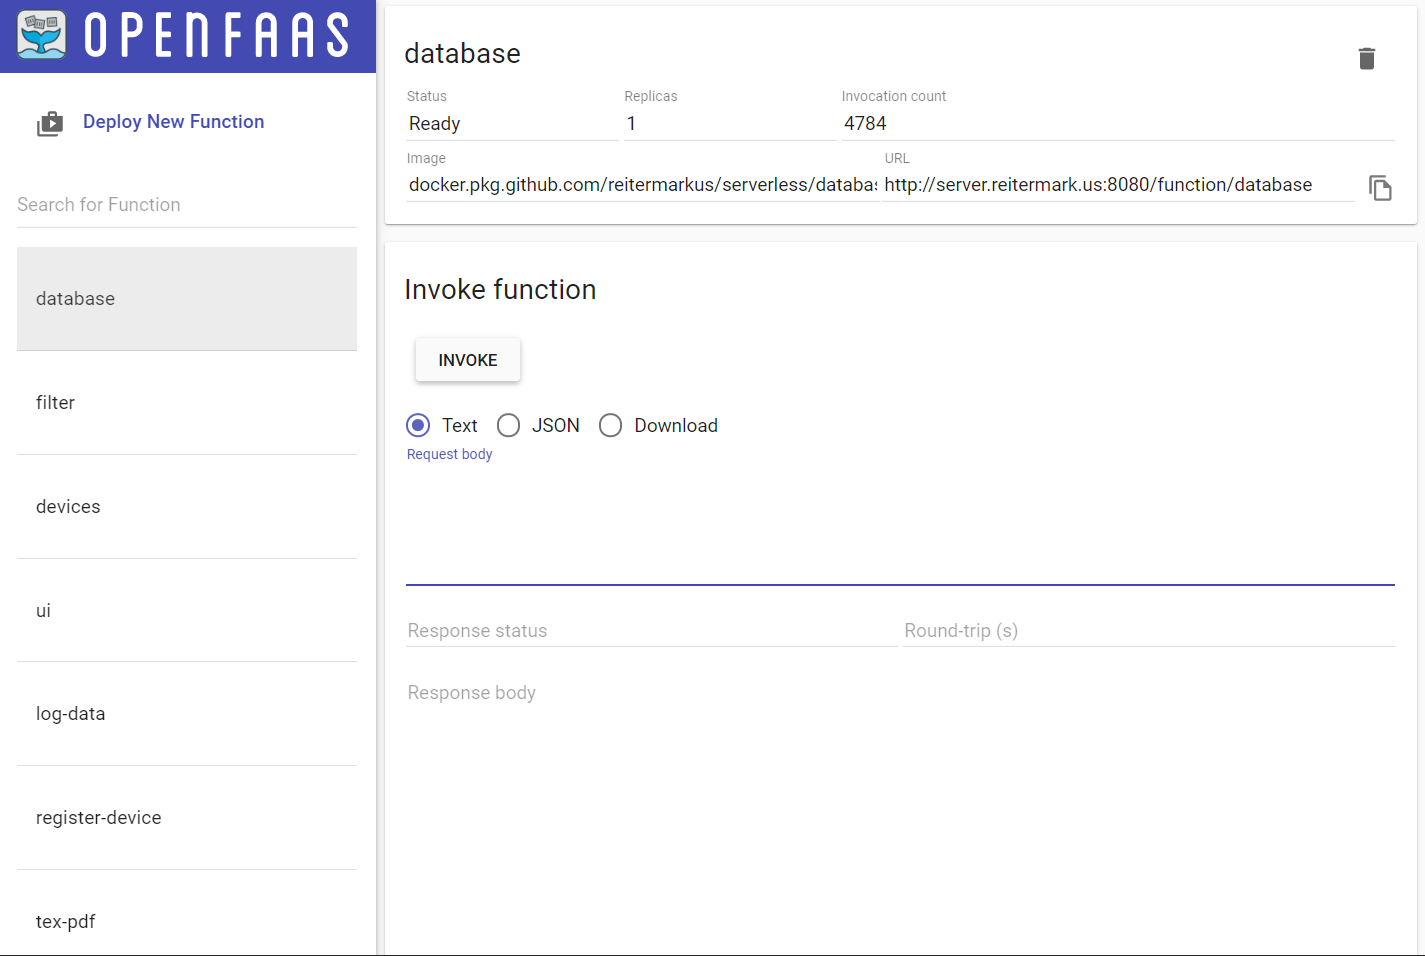
\includegraphics[height=15em]{openfaas-dashboard-small.png}
   \end{columns}
\end{frame}

\subsection{Functions}

With the OpenFaaS framework, every function consists of three parts: a function template, the
function's source code and a definition file.

Function templates are categorised by the programming language the corresponding function is written
in. At the bare minimum, a template contains a \texttt{Dockerfile} and a \texttt{template.yml}. The
\texttt{Dockerfile} has to be written in a way such that a \texttt{function} directory on the same
directory level is copied into the image. During the build step, this \texttt{function} directory
contains the source code, so depending on the programming language, it either has to be compiled or
moved to the correct location straight away. Additionally, the \texttt{Dockerfile} has to install
the \textit{OpenFaaS Watchdog}. The \textit{OpenFaaS Watchdog} is a service which is used to connect
the function to the \textit{OpenFaaS} gateway. Historically, the watchdog would pass requests to the
function via \textit{Standard Input} and return the function's \textit{Standard Output} as the
response. With this method however, the function could not control any aspect of the \textit{HTTP}
request and response. The new version of the \textit{OpenFaaS Watchdog} offers a few more operation
modes. The first, called \texttt{http}, forwards the received request to a specified port in the
function. This means that function templates using this mode have to be written in such a way that
they include a web server. This way the function can consume the \textit{HTTP} request directly,
which also makes calling functions easier since they can use standard \textit{HTTP} methods and
status codes. Another new mode is \texttt{static}, which can be used to create very simple functions
serving static files. \cite{of-watchdog} The \texttt{template.yml} file contains the metadata for
the function. This file can be empty, i.e. all metadata is optional, but most commonly it contains
at least the \texttt{language} property used to specify the programming language the template is
meant for. \cite{openfaas-build-functions} Commonly, a \texttt{function} directory containing a
“Hello, world!” function is included in the template itself to serve as a starting point when
creating a new function from scratch.

Another part needed for building a function is a definition file containing the name of the function
and all other data needed to deploy the functions. One essential part of this definition file is the
gateway URL, which the \textit{OpenFaaS Watchdog} uses to connect to the \textit{OpenFaaS} gateway.

\begin{code}[H]
  \centering
  \begin{lstlisting}
version: 1.0
provider:
  name: openfaas
  gateway: http://127.0.0.1:8080
functions:
  filter:
    lang: rust-http
    handler: ./filter
    image: filter:latest
    environment:
      RUST_LOG: info
      write_debug: 'true'
      gateway_url: http://gateway:8080
  \end{lstlisting}
  \caption{A definition file for a Rust function called \texttt{filter}.}
  \label{code:function-definition}
\end{code}

In \autoref{code:function-definition} we can see that there are two different gateway URLs. The first
one, \texttt{provider.gateway}, is used by the \texttt{faas-cli} command line tool in order to know
where to deploy the function to. The second one, \texttt{functions.filter.environment.gateway\_url}
is the URL the gateway can be reached from inside the cluster and the one passed to the
\textit{OpenFaaS Watchdog}. Furthermore, the function template is specified using
\texttt{functions.filter.lang}, the path the the function's source code is given by \\
\texttt{functions.filter.handler} and the name of the \textit{Docker} image is specified by \\
\texttt{functions.filter.image}.

Assuming the definition file shown in \autoref{code:function-definition} is called
\texttt{filter.yml}, we can build the function using the following command:

\begin{lstlisting}[language=bash]
faas-cli build -f filter.yml
\end{lstlisting}

Once built, the function can be deployed using an equally simple command:

\begin{lstlisting}[language=bash]
faas-cli deploy -f filter.yml
\end{lstlisting}

We chose to write all of our functions in Rust. When we first started, there was not yet an official
\textit{OpenFaaS} function template for Rust, so we had to create our own. For our custom template -
\texttt{Dockerfile} -, we used the builder pattern. In our case this meant, that we would first
compile the Rust function using the official \textit{Docker} image for \textit{Rust}. This image is
based on \textit{Debian}, which means that we could then copy the compiled function into a bare
\textit{Debian} image which doesn't include the \textit{Rust} compiler, therefore saving space. This
resulted in each function image being around \SI{90}{\mega\byte} in size. Still, this was too much
for a simple function in our opinion.

It is possible to write a \texttt{Dockerfile} without using any base image, using the \texttt{FROM
scratch} directive. For this to work, however, we need to generate a statically compiled version of
our functions since there is no operating system providing libraries. By extension, this meant, that
we had to replace our compile step, since the official \texttt{Rust} docker image does not provide
support for creating statically linked binaries. Thankfully, there exists a \textit{Docker} image
called \texttt{rust-musl-builder} \cite{rust-musl-builder} for this exact reason. Using the
\texttt{rust-musl-builder} image, we could reduce the average image size for our functions to around
\SI{15}{\mega\byte}, a sixth of their original size.

\subsubsection{The \texttt{database} Function}

One of the core building blocks of our project is the database, which stores information about
devices and is used for persistently storing the data received from those devices. For this reason,
naturally we needed a function which allows us to interact with the database.

We used the \href{https://github.com/mongodb/mongo-rust-driver}{\texttt{mongodb-rust-driver}}, a
Rust library for interfacing with a MongoDB database. In order to reduce latency, OpenFaaS keeps
functions running for a specified amount of time before considering them unused and terminating
them. This means that we only need to establish a connection to our database once, when the function
container is first started. Since the initial startup is handled by the function template and not
the function handler, we used the
\href{https://github.com/rust-lang-nursery/lazy-static.rs}{\texttt{laze\_static}} to lazily
initialise a static variable holding our database connection.

The actual function handler first parses a \textit{JSON} request containing either an
\texttt{insert}, \texttt{insert\_or\_update}, \texttt{find}, \texttt{aggregate} or \texttt{update}
action. These actions are then converted from \texttt{JSON} to \texttt{BSON} (Binary JSON), the
format MongoDB and by extension the MongoDB Rust driver uses. This allows other functions to call
this function in order to interact with the database instead of duplicating this logic in every
function which needs to access the database.

\subsubsection{The \texttt{register-device} Function}

The \texttt{register-device} function is used, as the name implies, to register new devices. This
function is triggered when a new message is posted to the \texttt{register-device} Kafka topic. The
function handler parses the message, which must contain a device ID and the device's name. If this
is the case, it then calls the \texttt{database} function in order to insert a new device or update
an existing device's name.

\subsubsection{The \texttt{log-data} Function}

Similarly to the \texttt{register-device} function, the \texttt{log-data} function is triggered when
a new message is posted to the \texttt{log-data} topic. A message is expected to contain a device
ID, the data type (e.g. humidity, pressure, etc.), the time the data was recorded as well as the
data itself. After parsing the message in the correct format, the function validates that the data
type is contained in a list of supported types, otherwise it responds with \textit{400 Bad Request}
error code. Afterwards, the \texttt{database} function is called in order to add the data type to
the list of supported data types of the given device. Then, another call to the \texttt{database}
function is made to insert the data in the collection for the corresponding data type.

\subsubsection{The \texttt{devices} Function}

The \texttt{devices} is probably the simplest function in our project. It calls the
\texttt{database} function to retrieve a list of all registered devices and their corresponding data
types, converts the list from \textit{BSON} to \textit{JSON} and then returns it. It is used by the
\textit{UI} for displaying a list of all devices.

\subsubsection{The \texttt{filter} Function}

Another function that is used by the \textit{UI} is the filter function. Given a device ID, it
returns the logged data for a specified data type. The function supports calculating averages for a
specified number of time slices in a given interval. To do this, we call our \texttt{database}
function with the \texttt{aggregate} function. In the request, we send the \texttt{begin},
\texttt{end} and \texttt{interval}. The logic for splitting this time frame into equally long chunks
resides in the \texttt{database} function itself. To collect the averages for each part, we first
calculate the difference between \texttt{begin} and \texttt{end} and then calculate the
\texttt{step} by dividing the difference by \texttt{interval}. We then loop, starting from
\texttt{begin} until we reach \texttt{end}, incrementing by \texttt{step} in each iteration.

\begin{code}[H]
  \begin{lstlisting}
'$match': {
  'time': {
    '$gte': ISODate('2020-02-26T18:23:00.000Z'),
    '$lte': ISODate('2020-02-26T21:53:00.000Z')
  }
}
  \end{lstlisting}
  \caption{A \textit{MongoDB} \texttt{\$match} statement filtering records with a \texttt{time}
  field containing a date between Feb. 26, 2020 18:23 and Feb. 26, 2020 21:53.}
  \label{code:mongodb-match}
\end{code}

As seen in \autoref{code:mongodb-match}, with \textit{MongoDB} it is very easy to retrieve records for a
given time span, using the \textit{\$match} pipeline operator.

\subsubsection{The \texttt{ui} Function}

Unlike many other functions, the \texttt{ui} function is not a \textit{Rust} function. Instead, it
utilises the new \textit{OpenFaaS Watchdog} mode called \texttt{static}. With it, we can create a
function solely consisting of static files. In the case of the \texttt{ui} function, these static
files are an \texttt{index.html}, a \texttt{style.css} and a \texttt{bundle.js}. Since our UI is
written purely in \textit{JavaScript}, we can use a single \texttt{webpack} command to produce all
these files. This process is explained in more detail in \autoref{sec:webpack}.

\subsubsection{The \texttt{tex-pdf} Function}

Like The \textit{ui} function, the \texttt{tex-pdf} function is also not a \textit{Rust} function.
This function is sort of a bonus, it is not required for the stack itself at all. \texttt{tex-pdf}
essentially queries the latest successful build from \textit{Azure}, tries to unpack the
\textit{PDF} in the \textit{thesis} artefact and finally display it in the browser. Therefore always
the latest version of the thesis will be served with the function and the user does not have to
compile the document with a \textit{LaTeX toolchain}.

\section{Raspberry Pi}

In order for us to gather data, we decided on using multiple \textit{Raspberry Pis} with different
sensors attached to them. We chose the \textit{Raspberry Pi} because it is backed by a huge
community and because of the vast amount of documentation available for it. Having documentation
available was essential, since we wanted to write the client application for the \textit{Raspberry
Pi} in \textit{Rust}. This way we could validate our \textit{Rust} code by comparing it to example
code written in other programming languages, most commonly \textit{Python} or \textit{C} in the case
of the \textit{Raspberry Pi}.

\subsection{\textit{Rust} on the \textit{Raspberry Pi}}

For our first “Hello, world!” program which would run on the \textit{Raspberry Pi}, we took the
simplest approach at the time. We would write the code on our development machines and synchronise
the code to the \textit{Raspberry Pi} using \texttt{rsync} \cite{rsync} and then compile and run it
via \texttt{ssh}. This worked fine at the time. Once we got to the point where we needed to add more
dependencies for the various sensors and networking, compile times naturally increased to the point
at which it simply wasn't feasible anymore to compile directly using the inadequate processor of the
\textit{Raspberry Pi}. A single build was approaching a compile time of around five minutes on every
single small change to the code, so we had to start looking for alternatives.

\subsection{Cross Compilation}

Soon after we realised that compiling directly on the \textit{Raspberry Pi} was not a good solution,
we had to find a way to cross compile for the \textit{Raspberry Pi}. This was further complicated by
the fact the we were using \textit{macOS} and \textit{Windows}, so none of the pre-compiled cross
compilation \whitelist{toolchains} for \textit{Linux} were an option for us.

We then found the \texttt{cross} \cite{cross} tool, which claimed to automatically install the
corresponding toolchain and then run the cross compilation in a \textit{Docker} container, so this
should have worked on both \textit{macOS} and \textit{Windows}. Right after we installed it using
\texttt{cargo install cross}, we saw that \textit{macOS} and \textit{Windows} support was lacking.
On both platforms, \texttt{cross} tried to simply call \texttt{cargo} directly instead of running in
a \textit{Docker} container. Since this tool still seemed to be the best solution we could find for
our situation and since the tool is open-source, we decided to dig into the source code and add the
missing \textit{macOS} and \textit{Windows} support ourselves.

Getting \texttt{cross} to actually run a \textit{Docker} container on both of our platforms was
quite easy, we only had to add two new definitions for \textit{Rust} toolchains in the source code
of \texttt{cross}, one for \textit{macOS} (\texttt{x86\_64-apple-darwin}) and one for
\textit{Windows} (\texttt{x86\_64-pc-windows-msvc}). The next problem we were facing was that inside
of the \textit{Docker} container, the \texttt{CARGO\_HOME} directory was mounted, and with it, its
\texttt{bin} subdirectory. This meant that the \textit{Docker} container would first look in this
directory instead of the respective toolchain root for the corresponding target's binaries. Since
the binaries in \texttt{CARGO\_HOME/bin} are compiled for the host machine, these previously worked
fine since only \texttt{x86\_64} \textit{Linux} hosts were supported. Now however, it would try
running a \textit{macOS} or \textit{Windows} binary inside of a \textit{Linux} \textit{Docker}
container. This was not as straight-forward to debug as it might seem, since the error message made
it seem as though it was a syntax error in a shell command. Once we found what the problem was, the
next challenge was to actually implement the fix for it. We still had to mount \texttt{CARGO\_HOME},
but exclude its \texttt{bin} subdirectory. Since the contents of \texttt{CARGO\_HOME} can vary
depending on what you have installed, we could not simply mount each subdirectory individually and
exclude \texttt{bin}, so the only way was to use a somewhat hacky workaround.

The whole \texttt{CARGO\_HOME} directory was already mounted using

\begin{lstlisting}[language=Bash]
-v "${CARGO_HOME}:/cargo:Z"
\end{lstlisting}

In order to prevent mounting the \texttt{bin} subdirectory from the host machine, we added

\begin{lstlisting}[language=Bash]
-v /cargo/bin
\end{lstlisting}

This means that technically the \texttt{bin} subdirectory is still mounted, but is overlaid by
another virtual volume which is not bound to a directory on the host, which effectively prevents
non-Linux binaries from being accessible inside the \textit{Docker} container. After this change, we could
finally compile our program on both \textit{macOS} and \textit{Windows}.

\subsection{Sensors}

For the actual collection of data, we of course needed to implement some sensors. The first sensor
we implemented is the widely used \textit{BMP180}, a digital sensor which acts as a combination of a
thermometer and barometer. The \\ \textit{BMP180} communicates over the \textit{I\textsuperscript{2}C}
bus. \textit{I\textsuperscript{2}C} is supported natively by most \textit{Linux} distributions,
consequentially also by the \textit{Raspbian} operating system running on the \textit{Raspberry Pi}.
We quickly found a \textit{Rust} library called \texttt{i2cdev}, which provides idiomatic wrapper functions
to interface with the \textit{Linux} \textit{I\textsuperscript{2}C} interface. Another library
called \texttt{i2cdev\_bmp180} then gave us an API for performing temperature and air pressure
measurements.

The second sensor we wanted to implement is the \textit{AM2320}, a digital temperature and humidity
sensor. The \textit{AM2320} also communicates over the \textit{I\textsuperscript{2}C} bus, which
means we could use a \textit{Rust} library fittingly called \textit{am2320}, which also is based on the
\textit{i2cdev} library, to produce temperature and humidity measurements. We also contributed some
improvements (see \url{https://github.com/gferon/am2320.rs/pull/1}) to this library.

The last sensor we implemented is a simple analogue photoresistor acting as a luminosity sensor. Due
to the fact that the \textit{Raspberry Pi} does not have any analogue \textit{GPIO} pins, we had to
resort to using an analogue-to-digital converter. To simplify the implementation of such a
converter, we chose the \textit{ADS1115}, which like the \textit{BMP180} and \textit{AM2320}
communicates over the \textit{I\textsuperscript{2}C} bus. With the \texttt{ads1x1x} library, we
could read the analogue photoresistor's voltage. By knowing this voltage, we can then
approximate the luminosity.

\begin{figure}[H]
  \centering
  \adjincludegraphics[max width=\textwidth]{wiring}
  \caption{Wiring diagram of sensors connected to a \textit{Raspberry Pi}}
  \label{fig:raspberry-wiring}
\end{figure}

In \autoref{fig:raspberry-wiring} we can see how the sensors are connected to the \textit{Raspberry
Pi}. The orange and red wires signify the 3.3V and 5V power supply lanes, respectively. The black
wire is the ground connection, and blue and violet are the two wires (receive/transmit) for the
\textit{I\textsuperscript{2}C} bus. From top to bottom, you can see the photoresistor connected to
the analogue-to-digital converter (ADC), followed by the \textit{BMP180} and the \textit{AM2320}. It
is easy to see that all sensors share the same \textit{I\textsuperscript{2}C} bus by looking at the
diagram.


\begin{frame}{Implementation -- Mobile Application}
  \begin{itemize}
    \item gyroscope
          \hspace*{18.4em}
          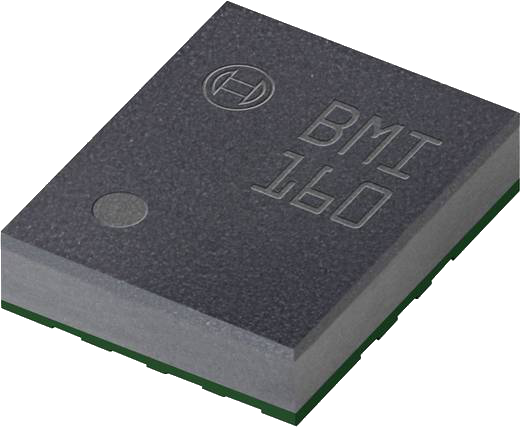
\includegraphics[align=c,height=3em]{bmi160-sensor}
    \item accelerometer
    \item magnetometer
    \item barometer
          \hspace*{18.4em}
          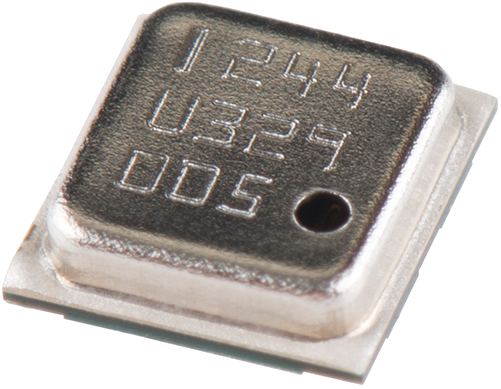
\includegraphics[align=c,height=3em]{barometric-sensor}
    \item gravity
    \item illuminance (only Android)
    \item proximity (only Android)
  \end{itemize}
\end{frame}

\begin{frame}{Implementation -- Mobile Application}
  \begin{columns}
    \column{0.5\textwidth}
      \begin{itemize}
        \item basic workflow
        \item difficulties with platform specific requirements
        \item fist try with React Native
        \item final Implementation in Flutter
        \item consists of five Views
      \end{itemize}
      \column{0.5\textwidth}
      \vfill
      \vspace*{2em}
      \centering
      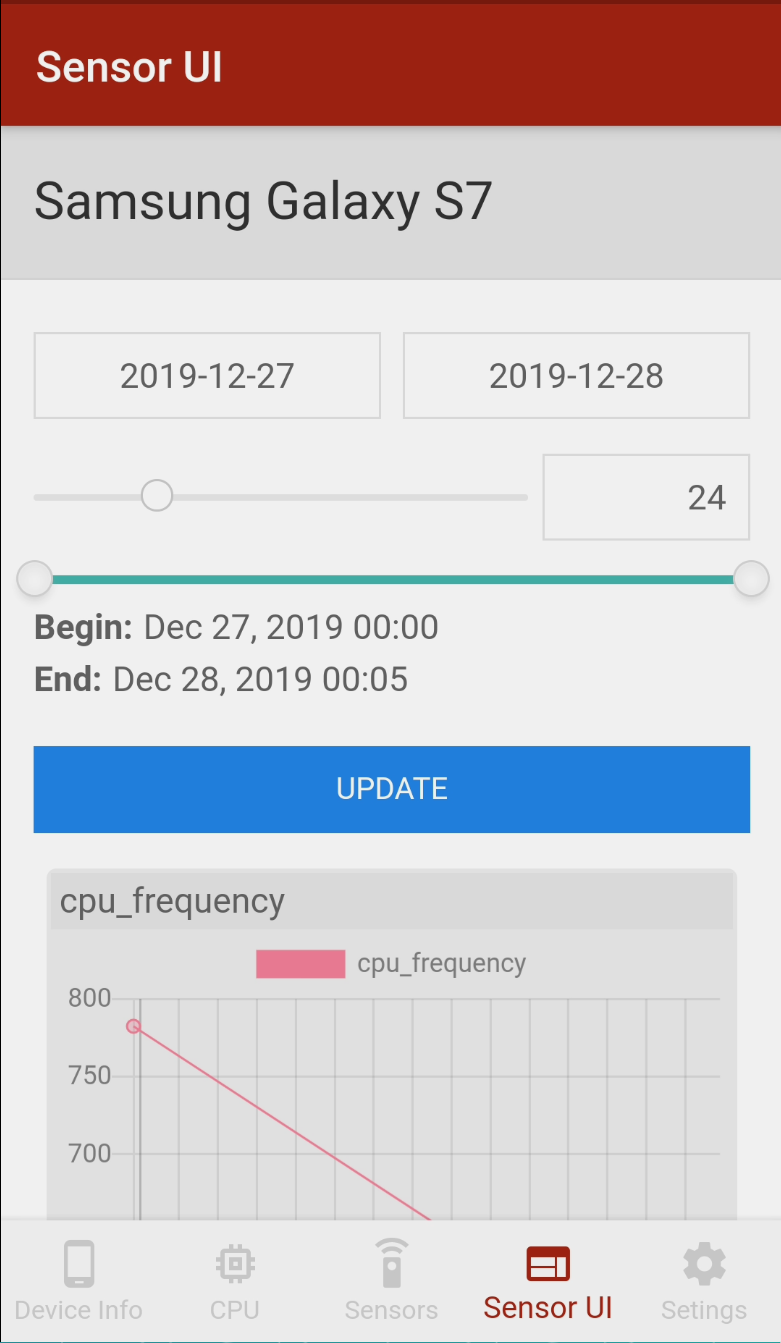
\includegraphics[height=16em]{mobile-sensor-ui.png}
   \end{columns}
\end{frame}

\begin{frame}{Implementation -- Mobile Application}
  \begin{columns}
    \column{0.25\textwidth}
    \vfill
    \vspace*{2em}
    \centering
    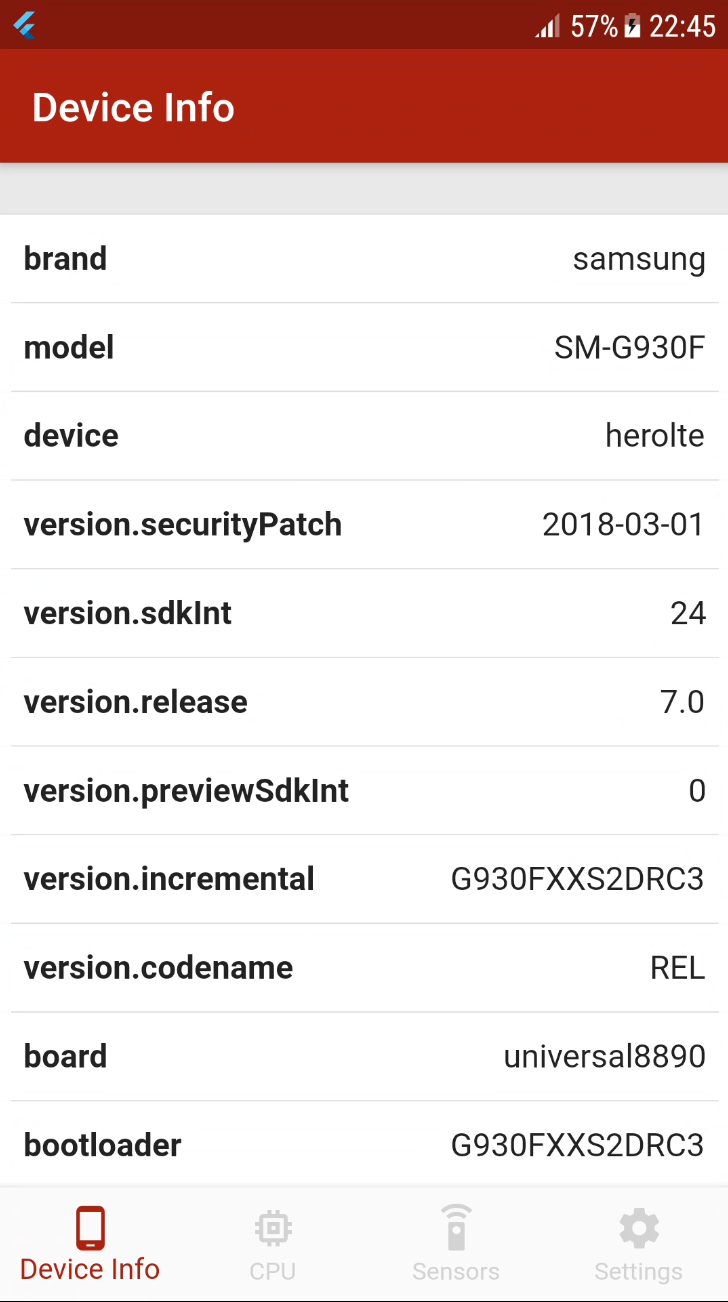
\includegraphics[height=16em]{mobile-device-info.png}

    \column{0.25\textwidth}
    \vfill
    \vspace*{2em}
    \centering
    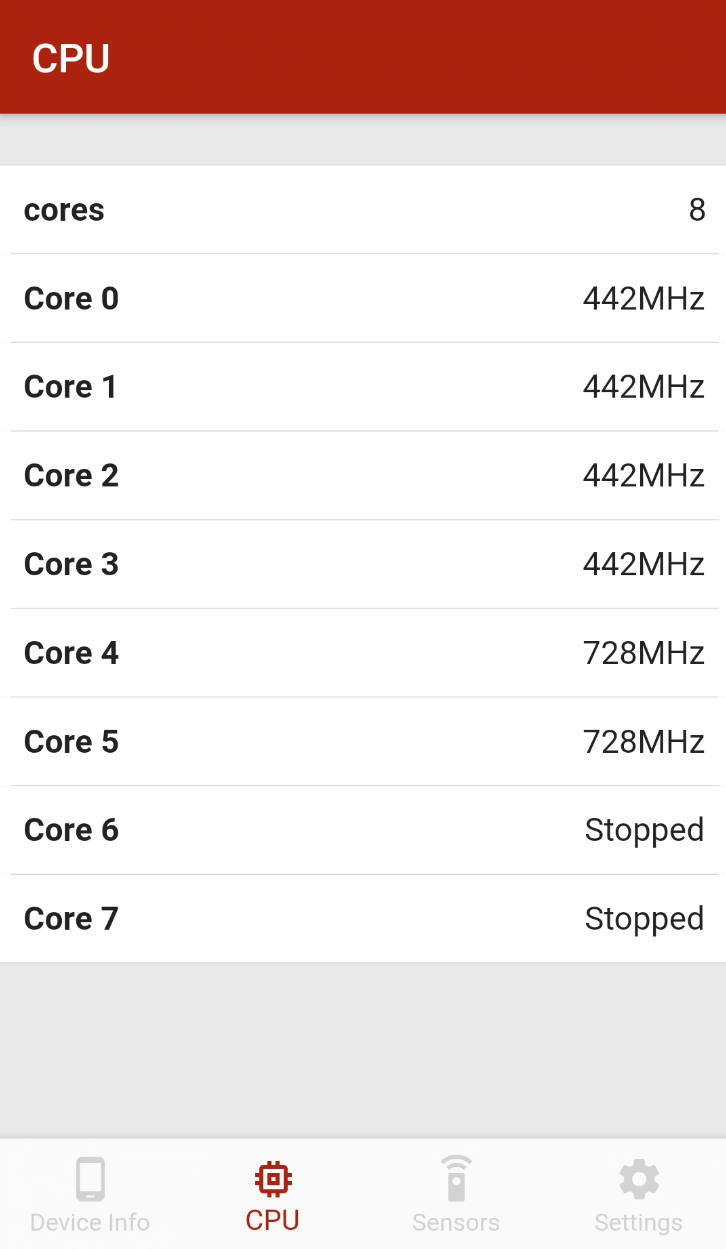
\includegraphics[height=16em]{mobile-cpu.png}

    \column{0.25\textwidth}
    \vfill
    \vspace*{2em}
    \centering
    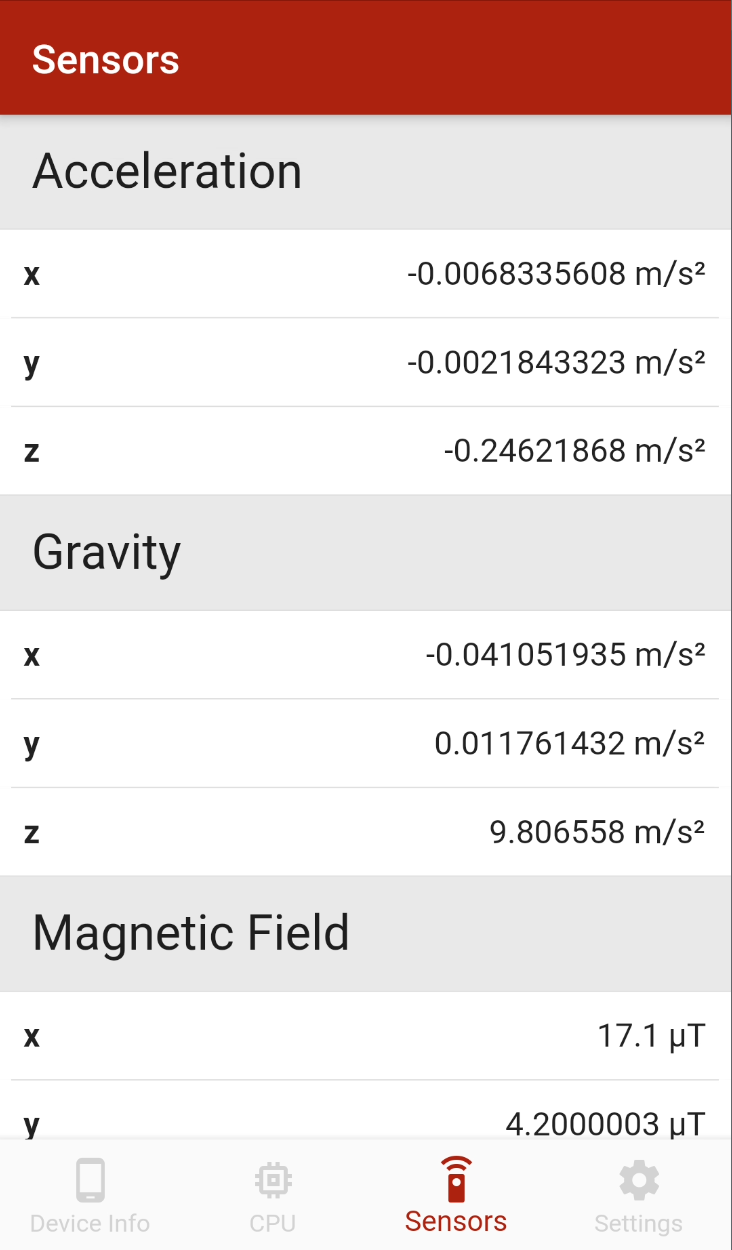
\includegraphics[height=16em]{mobile-sensors.png}

    \column{0.25\textwidth}
    \vfill
    \vspace*{2em}
    \centering
    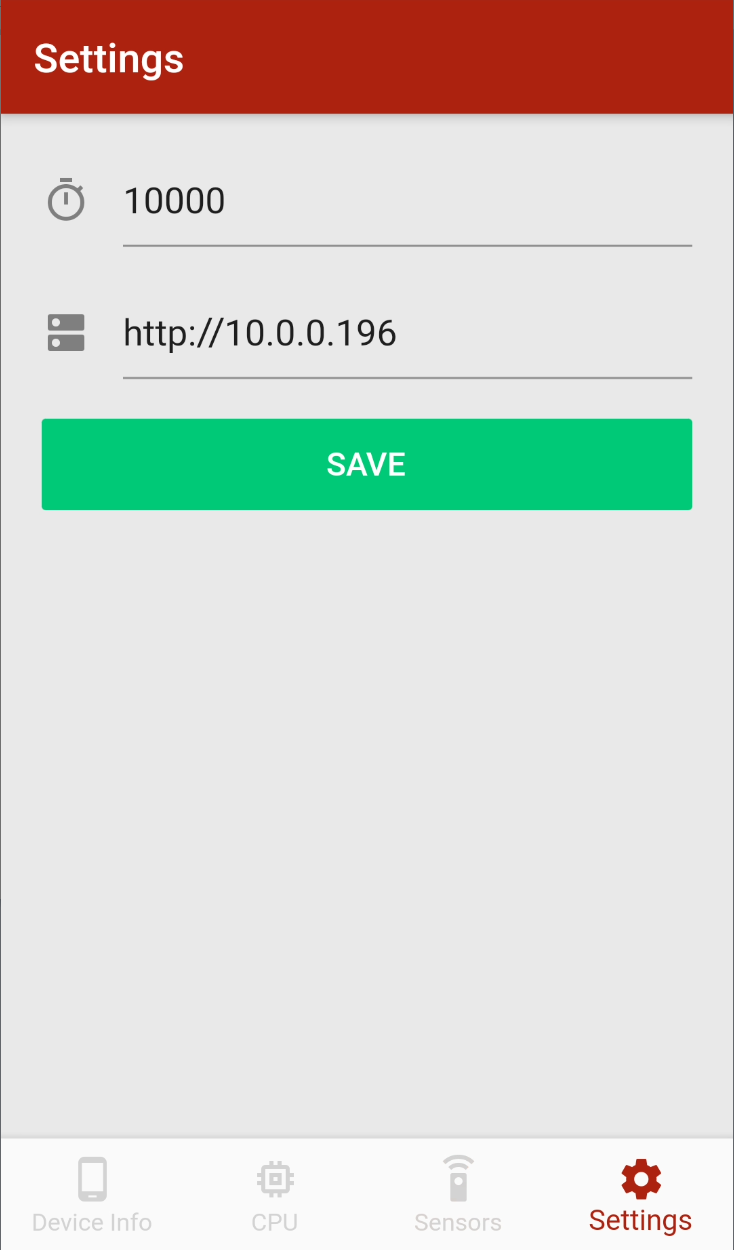
\includegraphics[height=16em]{mobile-settings.png}
  \end{columns}
\end{frame}

\begin{frame}{Implementation -- UI}
  \begin{columns}
    \column{0.35\textwidth}
      \begin{itemize}
        \item MarkoJS
        \item Babel
        \item Webpack
        \item SASS
      \end{itemize}
      \column{0.66\textwidth}
      \vfill
      \centering
      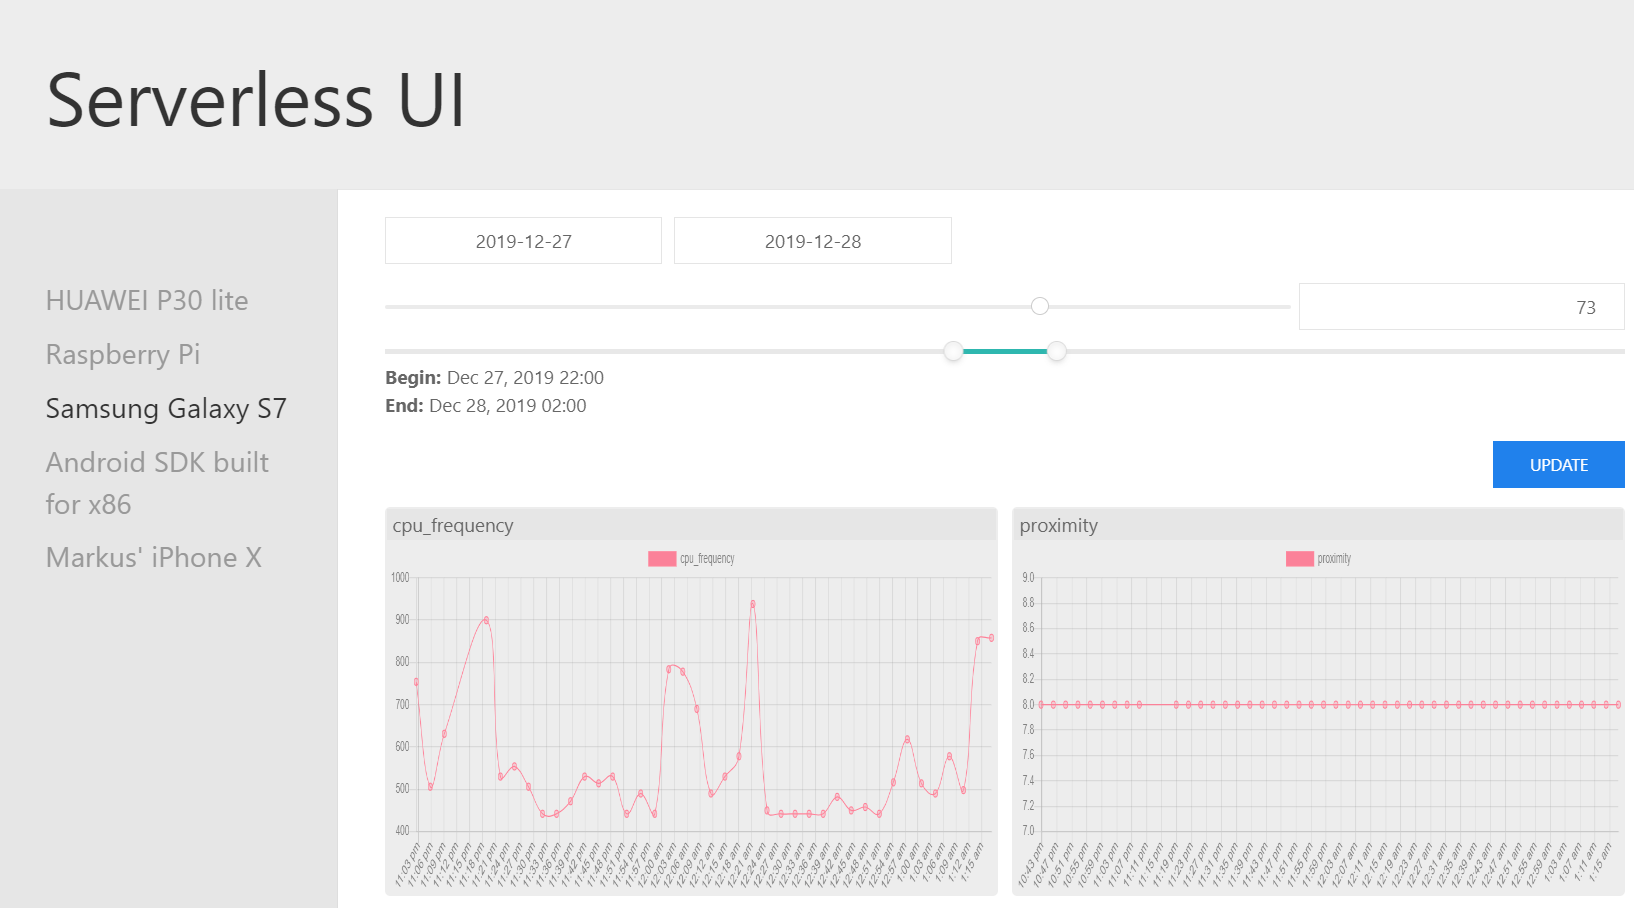
\includegraphics[width=24em]{serverless-ui-small.png}
   \end{columns}
  \end{frame}

  \begin{frame}{Implementation -- Mobile Application}
    \vfill
    \centering
    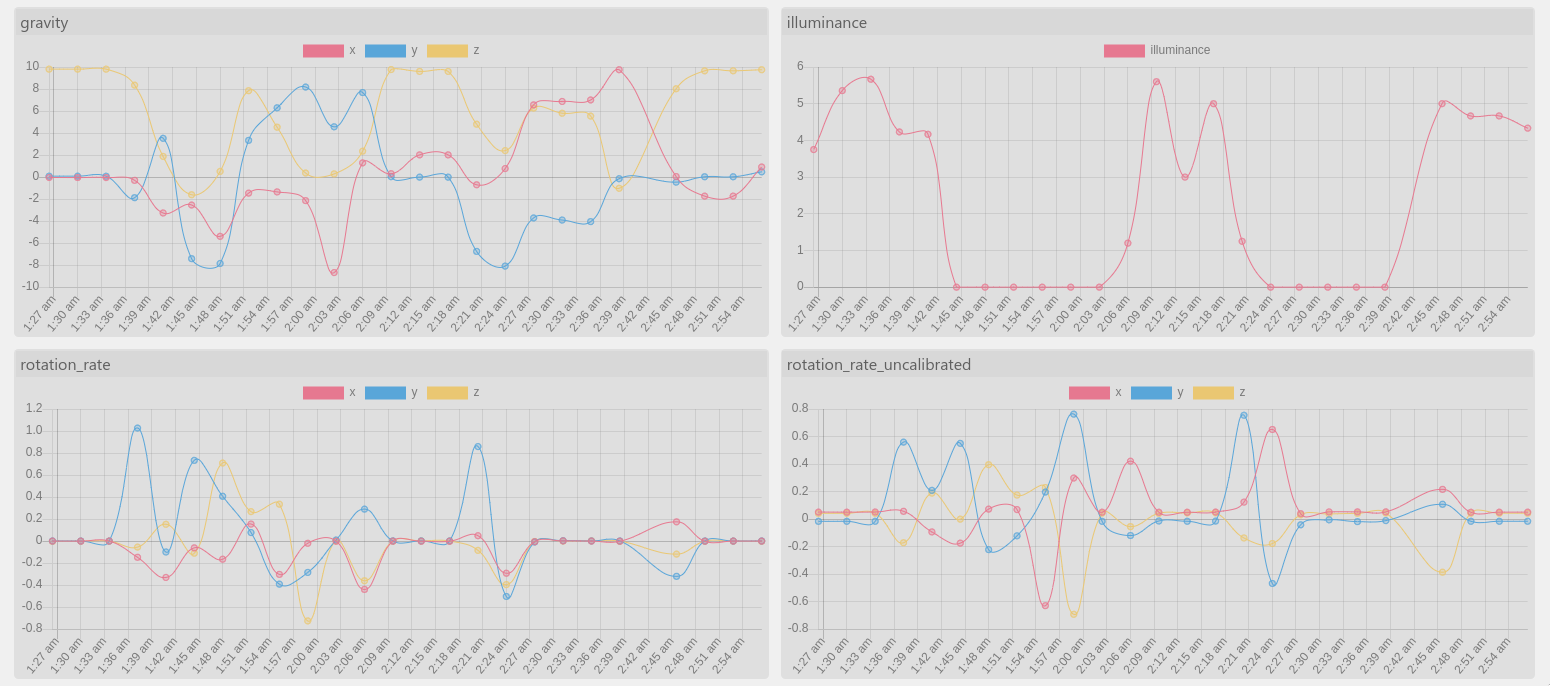
\includegraphics[height=16em]{ui-graphs.png}
  \end{frame}

  \newpage
  \chapter{Results}
\label{sec:results}

\section{Benchmarks}

For our test setup, we deployed our stack on an \textit{Intel NUC}, which is a fairly inexpensive
mini PC. With the following benchmarks, we want to show what such an affordable machine is capable
of when coupled with other cheap IoT devices, e.g. a Raspberry Pi.

\begin{table}[H]
  \centering
  \begin{tabular}{|l|l|l|r|}
    \hline
    Name                     & Model              & Processor                                                                             & Memory              \\ \hline
    \whitelist{Intel NUC}    & \whitelist{8I5BEH} & \whitelist{Intel Core i5-8259U} @ \SI{2.30}{\giga\hertz}                              & \SI{16}{\giga\byte} \\ \hline
    \whitelist{Raspberry Pi} & 3 B+               & \whitelist{Broadcom BCM2837B0, 64-bit SoC} @ \SI{1.4}{\giga\hertz}                    & \SI{1}{\giga\byte}  \\ \hline
    Desktop PC               & –                  & \whitelist{Intel Core i9-7900X} @ \SI{4.7}{\giga\hertz}                               & \SI{64}{\giga\byte} \\ \hline
  \end{tabular}
  \caption{Hardware used for Benchmark}
  \label{tab:benchmark-hardware}
\end{table}

The specific hardware we used for benchmarking is listed in \autoref{tab:benchmark-hardware} above.
The desktop PC and the \textit{NUC} were both connected via \whitelist{ethernet} to a \SI{1}{\giga\bit} network
switch. The \textit{Raspberry Pi} was connected via WiFi to an access point connected to the same
switch. \autoref{tab:benchmark-network-speed} shows the link speed between the hardware components
as tested with \texttt{iperf3} \cite{iperf}.

\begin{table}[H]
  \centering
  \begin{tabular}{|l|r|}
    \hline
    Connection                                  & Speed                          \\ \hline
    \textit{NUC} $\leftrightarrow$ Desktop PC   & \SI{940}{\mega\bit\per\second} \\ \hline
    \textit{NUC} $\leftrightarrow$ Raspberry Pi & \SI{55}{\mega\bit\per\second}  \\ \hline
  \end{tabular}
  \caption{Link speed between Hardware Components}
  \label{tab:benchmark-network-speed}
\end{table}


\begin{table}[H]
  \centering
  \begin{tabular}{|r|r|}
    \hline
    Number of Sensors & Messages per Second \\ \hline
                    1 &                7.55 \\ \hline
                    8 &               49.20 \\ \hline
  \end{tabular}
  \caption{Benchmark for Messages per Second from a Raspberry Pi to a \whitelist{NUC}}
  \label{tab:benchmark-nuc-raspberry-pi}
\end{table}

In \autoref{tab:benchmark-nuc-raspberry-pi}, we see the benchmark data for the \texttt{log-data}
function. For this benchmark, we set the \textit{Raspberry Pi} to not use any delay between
measurements instead of the usual measurement interval of \SI{15}{\second}. We also disabled the
\texttt{CPU Load Aggregate} measurement, since this has an inherent delay of \SI{1}{\second} due to
the fact that it calculates the load average for a given duration. The \textit{Raspberry Pi}
application collects the data for all sensors in each iteration, which means that we can actually
get much more throughput with eight sensors than with a single sensor. Thus, we can further
conclude that the time to produce a measurement is negligible compared to the network latency.

In order to test this theory, we decided to use parallel \texttt{curl} requests from a more
powerful computer to test the limit of the \textit{NUC}.

\begin{table}[H]
  \centering
  \begin{tabular}{|r|r|}
    \hline
    Number of concurrent Requests & Messages per Second \\ \hline
                                1 &                61.2 \\ \hline
                               10 &               239.0 \\ \hline
                               20 &               322.4 \\ \hline
                               50 &               379.5 \\ \hline
  \end{tabular}
  \caption{Benchmark for Messages per Second from a Desktop PC to a \whitelist{NUC}}
  \label{tab:benchmark-nuc-curl}
\end{table}

Each \texttt{curl} request in \autoref{tab:benchmark-nuc-curl} contains a single sensor record which
corresponds to the case in \autoref{tab:benchmark-nuc-raspberry-pi} with a single sensor. By looking
at this data, we can see when only sending data for a single sensor, the \textit{Raspberry Pi} is
clearly the bottleneck, not the \textit{NUC}. It is safe to assume that the \textit{NUC} is able to
handle approximately 400~requests per second.

With this assumption that a \textit{NUC} can handle 400~requests per second, we can deduce that with
our test setup, we are able to process streams from between

$\frac{400}{7.55} \times 1 \approx 53$

and

$\frac{400}{49.20} \times 8 \approx 65$

sensors.

This being a synthetic benchmark, it is likely that in a real world scenario, where sensor data is
sent only every \textit{x} seconds, the number of supported sensors is actually in the~100s instead
of only in the~10s.

  \newpage
  \section{Conclusion and Future Work}
\label{sec:conclusion}

As explained in the thesis, building an infrastructure like the one we have is not a trivial task
and requires an extensive amount of research. The final result then however shows the flexibility
and benefits of our stack and by extension of \textit{Serverless Computing}. It is trivial to switch
the programming environment as one only has to write a new function and provide a corresponding
\textit{Dockerfile}. In terms of \textit{IoT} devices, \textit{FaaS} seems to be a fitting concept
as well, since it offers high scalability and parallelism of invocations, which means the stack can
support an arbitrary amount of devices and is mostly only limited by the hardware it is running on.
While \textit{Kafka} adds a bit of overhead, its managing capabilities are especially useful in the
case of a high amount of connected clients. The choice of a host for persisting data in a project
like this is also very important. \textit{MongoDB} proves to be capable in that regard. Its
\textit{JSON} inspired documents make it easy for devices with low hardware specifications to
process data as representing data with \textit{JSON} is straight forward. Unfortunately the same
cannot be said when dealing with mobile applications in a \textit{cross platform} way. The
\textit{cross platform} aspect in our project is essentially limited to the user interface. Newer
versions of both \textit{Android} and \textit{iOS} do not work well when confronted with the
requirement of always having to send data in the background, as both platforms impose energy saving
restrictions and therefore prevent the application from working as intended.

Ultimately, our project is supposed to act more as a proof of concept and give an insight what could
be possible with this kind of technology. Although the mobile application is not ideal from a
usability standpoint as mentioned before. From the standpoint of our \textit{OpenFaaS} stack
however, it is also a success as it shows the capability of the infrastructure of dealing with
various different devices. Our project can therefore be used as a basis for future work as there is
still room for improvement, especially in the latency department. The technology of
\textit{Serverless Computing} seems to be more suited for deployment on a larger scale where many
devices send data at the same time. Optimising throughput is not the only thing that still can be
done. Security aspects like roles and authorisation could also be imposed in order to control who
and which device is allowed to call a function.


  \newpage
  \printbibliography

  \newpage
  \appendix
\appendixpage
\addappheadtotoc

\section{Rakefile}

\subsection{\texttt{deploy:functions}}
\lstinputlisting[
  language   = Ruby,
  linerange  = {
    namespace\ deploy\ begin,
    functions,
    namespace\ deploy\ end
  },
]{../../Rakefile}

\newpage
\subsection{\texttt{deploy:swarm}}
\lstinputlisting[
  language  = Ruby,
  linerange = {
    namespace\ deploy\ begin,
    swarm,
    namespace\ deploy\ end
  },
]{../../Rakefile}

\end{document}
